\documentclass[11pt]{article}
\usepackage[a4paper,left=22mm,right=22mm,top=23mm,bottom=25mm]{geometry}
\usepackage{graphicx}
\usepackage{url}
\usepackage{hyperref}
\usepackage{amsmath}
\usepackage{fancyhdr}
\usepackage[utf8]{inputenc}
\hypersetup{colorlinks=true,linkcolor=blue,urlcolor=blue}

\begin{document}
\clubpenalty 10000
\widowpenalty 10000

\title{3. Experimentální hodnocení kvality algoritmů}
\author{Ladislav Martínek}
\date{}
\maketitle
 
\section{Zadání úlohy} 

\begin{itemize}
\item Prozkoumejte citlivost metod řešení \href{http://www.csc.kth.se/~viggo/wwwcompendium/node211.html#7374}{problému batohu} na parametry instancí generovaných generátorem náhodných instancí. Máte-li podezření na další závislosti, modifikujte zdrojový tvar generátoru.
\item Na základě zjištění navrhněte a proveďte experimentální vyhodnocení kvality řešení a výpočetní náročnosti
\item Zkoumejte zejména následující metody
\begin{enumerate}
\item hrubá síla (pokud z implementace není evidentní úplná necitlivost na vlastnosti instancí)
\item metoda větví a hranic, případně ve více variantách
\item dynamické programování (dekompozice podle ceny a/nebo hmotnosti). FPTAS algoritmus není nutné testovat, pouze pokud by bylo podezření na jiné chování, než DP
\item heuristika - poměr cena/váha
\end{enumerate}
\item Pozorujte zejména závislosti výpočetního času (případně počtu testovaných stavů) a rel. chyby (v případě heuristiky) na:
\begin{enumerate}
\item maximální váze věcí
\item maximální ceně věcí
\item poměru kapacity batohu k sumární váze
\item granularitě (pozor - zde si uvědomte smysl exponentu granularity)
\end{enumerate}
\item Doporučuje se zafixovat všechny parametry na konstantní hodnotu a vždy plynule měnit jeden parametr. Je nutné naměřit výsledky pro aspoň čtyři (opravdu minimálně) vhodně zvolené hodnoty parametru, jinak některé závislosti nebude možné vypozorovat.
\end{itemize}

\section{Rozbor řešení}\label{kap:1}
Pro určení a sledování citlivosti na různé instance problému jsem využil generátor náhodných instancí, u které lze nastavovat jednotlivé parametry. U instancí problému jsou nastavovány parametry jako granulalita, maximální cena, maximální váha a poměr sumární váhy ke kapacitě batohu. Pokusím se odhadnout chování algoritmů při změnách parametrů jednotlivých instancí. Tedy sledovat citlivost algoritmů na dané parametry. 
\subsection{Metoda hrubé síly}
Medota hrubé síly nebude v tomto experimentu zkoumána, protože je zřejmé, že pokaždé projde všechny instance a tedy vubec není citlivá na jiné parametry, kromě paramentru n, který ale již by prozkoumán v 1. a 2. úloze.


\subsection{Metoda větví a hranic (B\&B)} 
U této metody očekávám velkou čitlivost na poměr celkové váhy a kapacity batohu, dále by metody mohla ovlivnit granularita. Tato metoda nemá horní mez a proto její čas může narůst až na metody hrubé síly. 

\subsection{Metody dynamického programování (obě dekompozice)}
U dekompozic očekávám citlivost vždy na daný parametr. U dekompozice podle ceny tedy citlivost na maximální cenu a u dekompozice podle váhy na maximální váhu. 

\subsection{Řešení heuristikou poměr cena/váha}
Očekávám, že heuristická metoda bude datově citlivá a to především na paramentry jako poměr celkové váhy a kapacity batohu nebo granularita. Vliv maximální ceny a váhy neočekávám.




\section{Popis kostry algoritmu}\label{kap:2}
Všechny algoritmy a průběh experimentu, zůstali stejné jako v úloze 2. Byli pouze změněny soubory s instancemi, které byli vygenerovány před experimentem.


\section{Experimenty}
 
Experimenty jsem prováděl v režimu jednoho vlákna na starším datovém serveru v podobě starého notebooku, který v době výpočtu nebyl používán. Výsledky tedy nejsou ovlivněny jinými běžícími programy. Procesor na testovacím stroji: \textit{Intel Pentium T3400 (2 cores). Taktován na 2.16~GHz s~1~MB cache}.
Měření času CPU probíhalo v knihovně $timeit$ s několika násobným průchodem pro menší instance. Pro každý parametr bylo vygenerováno 100 instancí.




\subsection{Závislost na poměru součtu vah předmětů k nosnosti batohu}
\subsection{Závislost na maximální ceně předmětů}
\subsection{Závislost na maximální váze předmětů}
\subsection{Závislost na granularitě instance}



\begin{figure}[h]\centering
	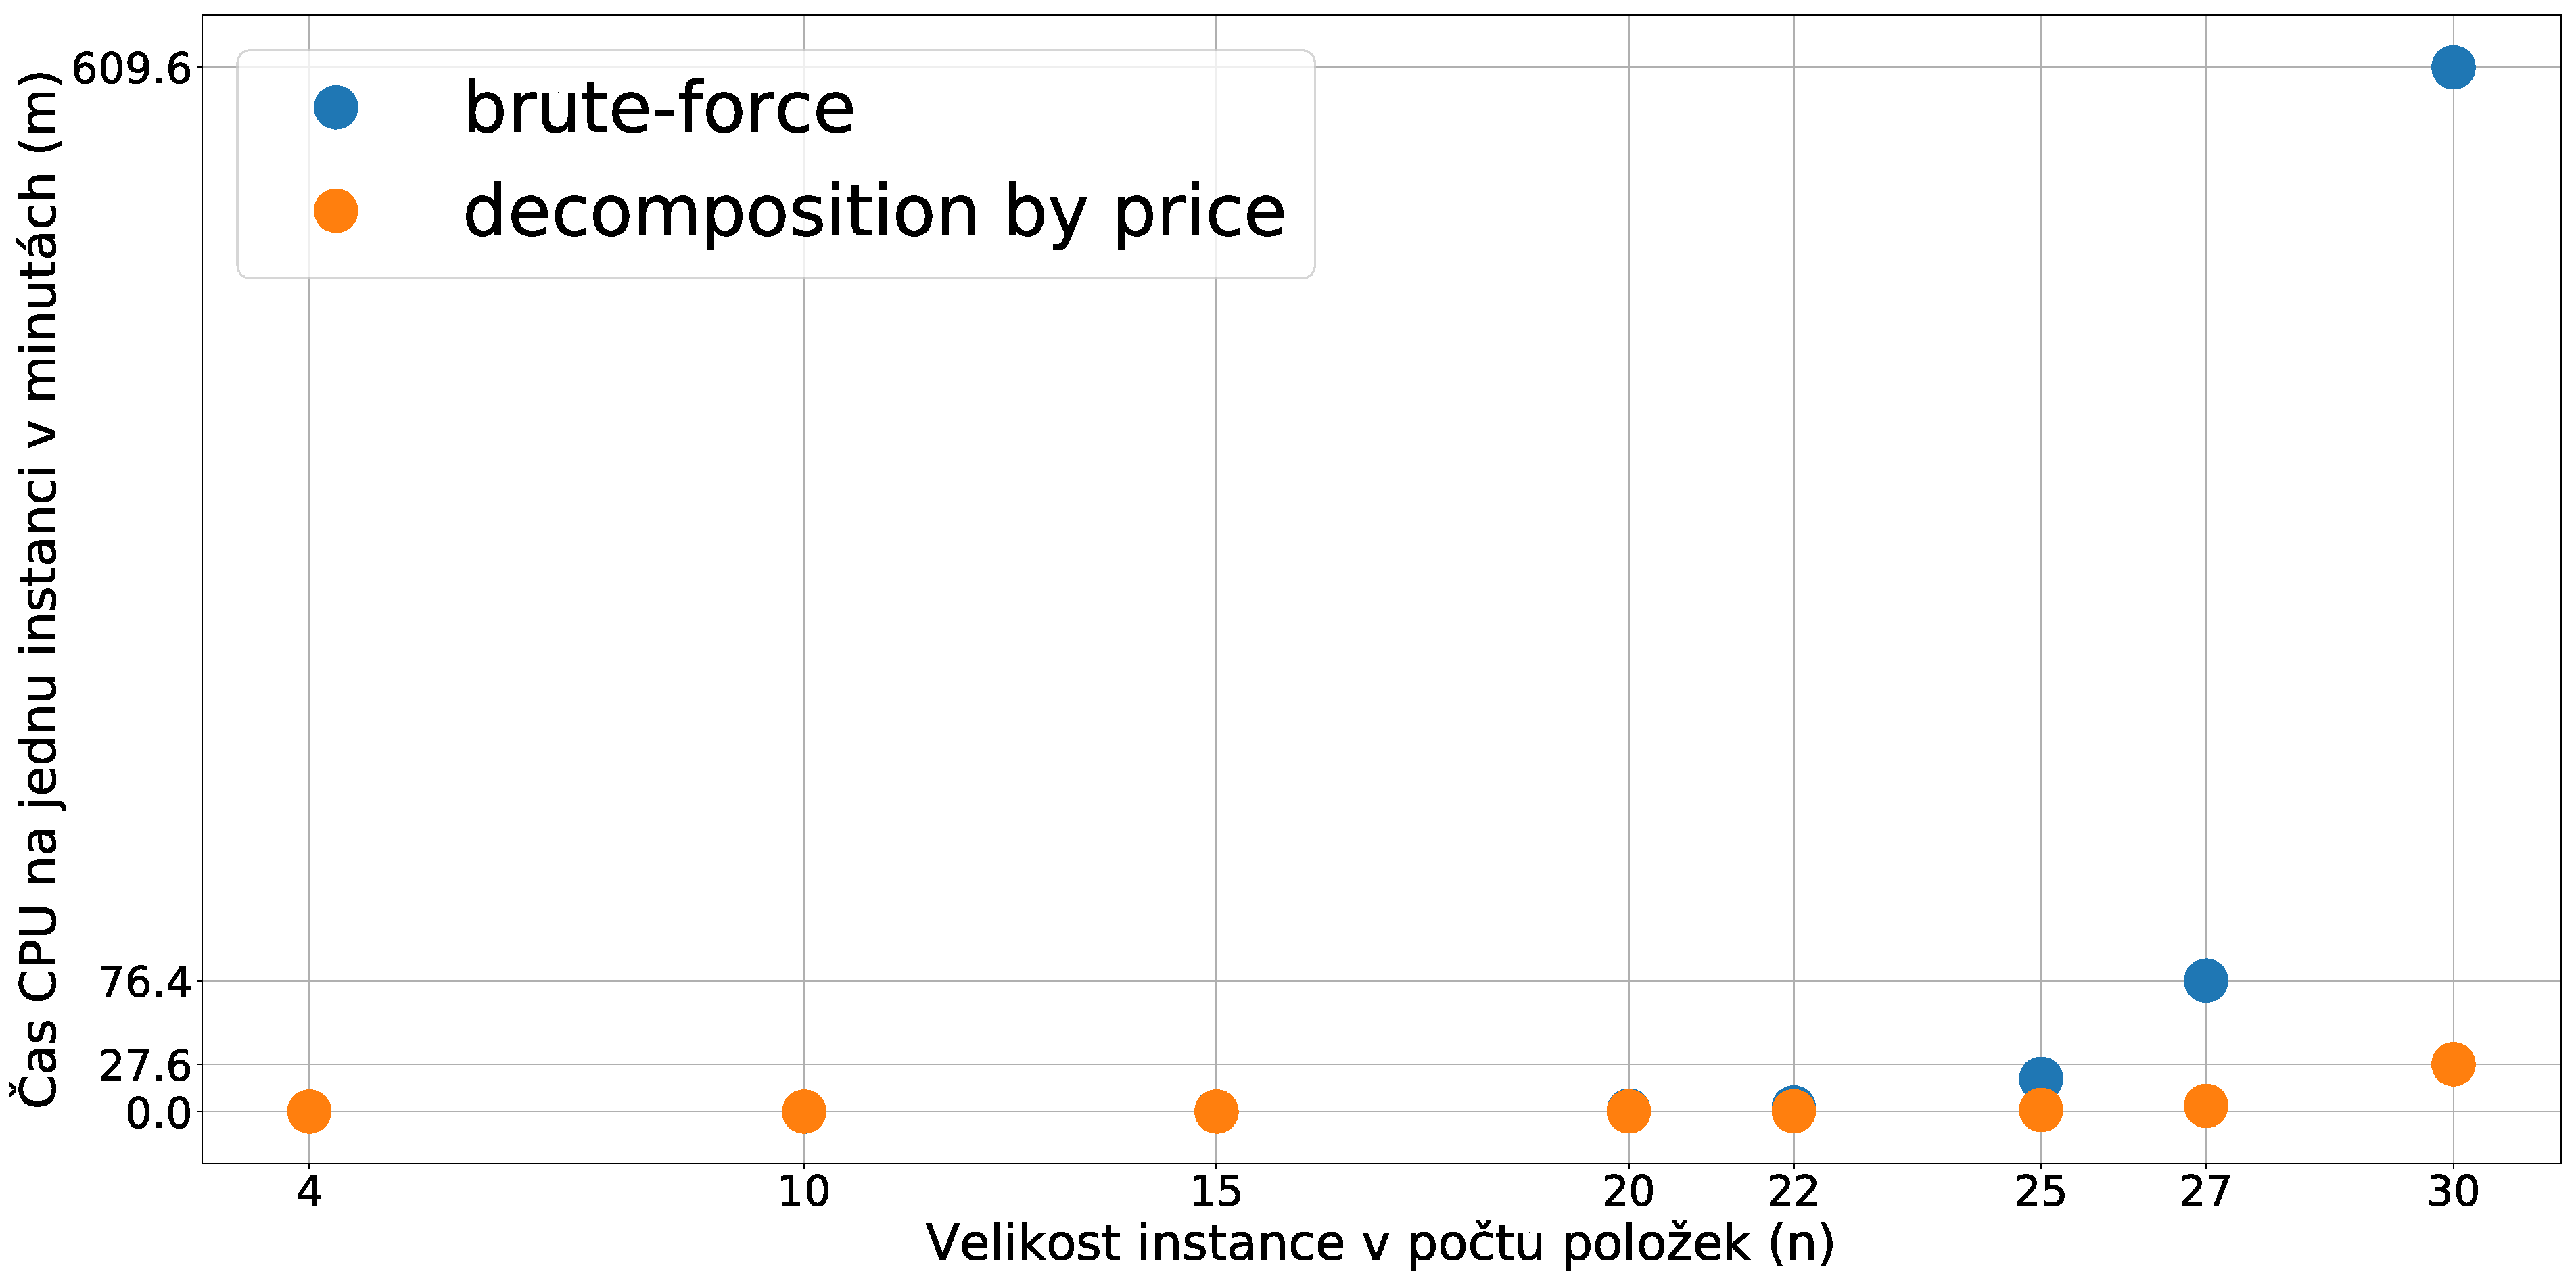
\includegraphics[scale=0.2]{img/tBavg}
 	\caption[1]{Brute-force ve srovnání s dynamickým programováním s dekompozicí podle ceny. Časová náročnost. Na grafu jsou průměrné hodnoty.}\label{fig:1}
 \end{figure} 	


\section{Závěr}
Během experimentu jsem otestoval velké množství instancí s různými parametry a sledoval citlivost algoritmů na tyto parametry. Byli pozorovány časy exaktních algoritmů a u heuristiky byla také měřena relativní chyba. 


\end{document}